\part{Généralités}

\section*{Remarques générales}

\begin{itemize}
 \setlength\itemsep{3pt}
 \item \textbf{Niveau du binôme :} Intermédiaire
 \item \textbf{Adresse du dépôt Git :} \url{https://github.com/GCoiffier/Projet-2}
 \item Les fichiers de tests sont situés dans le dossier Programs. Les fichiers contenant du code fouine ont une extension \texttt{.ml}
 \item Les fichiers compilés pour la machine SECD sont situés dans le dossier Stack\_Programs. Ils ont une extension \texttt{.code}
 \end{itemize}

\section{Comment exécuter notre programme}

\subsection{Avec Linux}

\begin{itemize}
  \setlength\itemsep{3pt}
 \item Pour compiler le programme, utilisez simplement la commande \texttt{make}. Celle-ci crée un exécutable appelé \textit{fouine}.
 \item Pour nettoyer le répertoire de travail, utilisez la commande `make clean`.
 \item \texttt{./fouine fichier} exécute le code contenu dans **fichier** et renvoie le résultat de ce code (qui doit être un entier)
 \item \texttt{./fouine -debug fichier} commence par afficher le code parsé dans la console, puis exécute le code et affiche le résultat.
 \item \texttt{./fouine -interm sortie fichier} compile le code parsé et le stocke dans sortie. Si aucun fichier de sortie n'est spécifié, le programme affichera le code dans la console.
 \item \texttt{./fouine -machine fichier} compile le code parsé et effectue l'interprétation mixte : ce qui peut être exécuté sur la machine à pile y est exécuté, le reste fait appel à l'interpréteur standard. Le code en entrée doit être un code fouine.
 \item \texttt{./fouine -execute fichier} compile le code parsé et l'exécute sur la machine à pile. Ce code doit être dans le langage de la machine à pile.
 \item \textbf{NB :} il est dans tous les cas possibles de ne pas donner de fichier d'entrée à fouine. Le programme s'éxecute alors en mode interactif et il faut entrer un programme dans la console.
\end{itemize}

\paragraph{Exemples :}

\texttt{
\begin{itemize}
 \setlength\itemsep{3pt}
 \item[>] ./fouine
 \item[>] ./fouine Programs/factorielle.ml
 \item[>] ./fouine -debug Programs/function.ml
 \item[>] ./fouine -interm
 \item[>] ./fouine -interm toto.code Programs/prog1.ml
 \item[>] ./fouine -execute toto.code
 \item[>] ./fouine -machine Programs/prog2.ml
 \item[>] ./fouine -debug Programs/function.ml
\end{itemize}
}

\subsection{Avec un autre OS}

\begin{enumerate}
 \item Installez Linux
 \item Reprendre les instructions de la section précédente.
\end{enumerate}


\section{Fouine}

\subsection{Fouine}
La fouine (Martes foina) est une espèce de mammifères carnivores d'Europe et d'Asie, au pelage gris-brun, courte sur patte et de mœurs nocturnes. C'est une martre (ou marte) faisant partie de la famille des Mustélidés, au même titre que la belette, le blaireau, la loutre, le putois ou le furet, petits mammifères carnivores se caractérisant souvent par leur odeur forte.

\begin{figure}[ht]
\centering
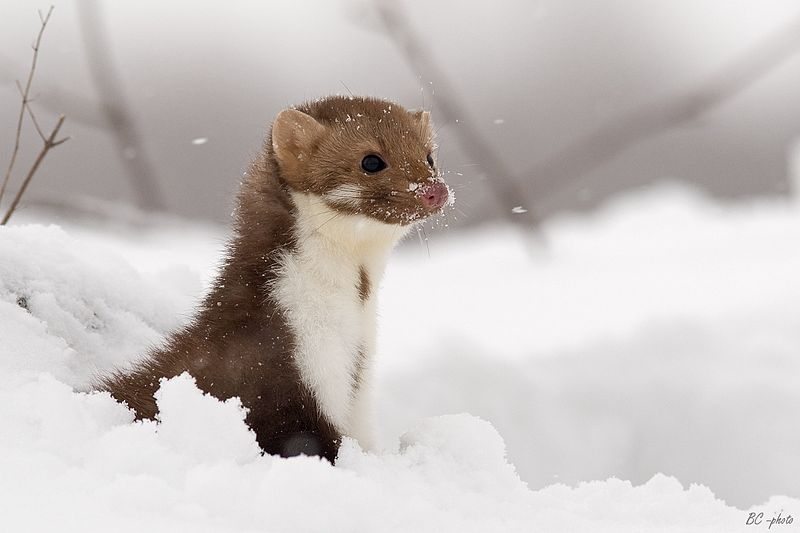
\includegraphics[width=8cm]{fouine_hiver.jpg}
\caption{Fouine photographiée en hiver en République tchèque.}
\end{figure}

Les fouines sont des animaux solitaires, comme la plupart des autres espèces de martres. Elles évitent leurs congénères en dehors des périodes de reproduction. Il s'agit d'animaux territoriaux qui marquent leur territoire avec des secrétions et le défendent au moins contre d'autres fouines de même sexe. La grandeur du territoire est variable, mais reste inférieure à celui de la Martre des pins. Leur grandeur va de 12 à 21cm et varie en fonction du sexe (les territoires des mâles sont plus grands que ceux des femelles), de la saison (ils sont plus petits en hiver), de l'habitat (ils sont plus grands en campagne qu'en ville) et de la nourriture disponible. Leur activité est surtout nocturne. L’espérance de vie de la fouine est d’approximativement douze ans. \\ ~ \\

\textit{Extraits de l'article de Wikipedia \cite{WikiFouine}}

\subsection{Le langage Fouine}

Le langage fouine est un langage de programmation constituant un sous-ensemble du langage Ocaml. Il comprend notamment :
\begin{itemize}
 \item Les expressions arithmétiques et booléennes
 \item Les déclarations de variables et de fonction (syntaxe \texttt{let ... = ... in ...})
 \item Les branchements conditionnels
 \item Les fonctions récursives (syntaxe \texttt{let rec ... = ... in ...})
\end{itemize}

Mais, à la différence d'Ocaml, il ne comprend pas :
\begin{itemize}
 \item De typage : toutes les fonctions prennent en argument des entiers, et renvoient des entiers
 \item De structures de données telles que les listes
 \item De filtrage par motif
 \item La couche orientée objet
\end{itemize}

Cependant, nous verrons que fouine peut être étendu avec certaines fonctionnalités, notamment un système de gestion d'exceptions et des références.\\
Ce langage ne figure cependant pas dans la liste des 700 langages de programmation proposée par Peter J. Landin \cite{700}.

\section{Organisation du rapport et du projet}

\subsection{Organisation du rapport}

Ce rapport s'organise en 3 parties, si l'on exclut cette partie d'introduction. \\
Dans un premier temps, nous parlerons de l'interpréteur fouine, de ses fonctionnalités et de certains aspects importants de son implémentation. \\
Dans un second temps, nous parlerons de la machine à pile SECD, également implémentée par nos soins. \\
Enfin, la dernière partie sera consacrée à l'exécution mixte fouine/SECD d'un code.

\subsection{Organisation du projet}



\subsection{Avancement du projet en fonction du temps}
\subsubsection*{Rendu 2}
\begin{itemize}
 \item \textbf{Semaine 1} 
    \begin{itemize}
    \item Lexer et parser de base

    \item Définition d'un type programme pour les programmes fouine

    \item Interprétation des fichiers fouine sans les fonctions
      (ie expressions arithmétiques, booléennes, \texttt{if ... then ... else} et \texttt{let ... in})
    \end{itemize}
    
  \item \textbf{Semaine 2 }
    \begin{itemize}
      \item Interprétation des fichiers fouine avec des fonctions
      \item Interprétation des fichiers fouine avec des fonctions récursives
    \end{itemize}
  
  \item \textbf{ Semaine 3 }
    \begin{itemize}
    \item Gestion des exceptions
    \item Gestion des références
    \item Gestion du \texttt{begin...end} et du \texttt{let \_ = ...}
    \item Ajout de primitives "bonus" \texttt{prStr} (qui renvoie 0 et affiche une string) et \texttt{prNl} (qui passe une ligne et renvoie aussi 0)
    \end{itemize}
\end{itemize}

\subsubsection*{Rendu 3}
\begin{itemize}
 \item \textbf{Semaine 4 }
    \begin{itemize}
      \item Correction des exceptions (on utilise plus \texttt{try ... with} de Caml)
      \item Implémentation des tableaux
      \item Compilation des expressions arithmétiques vers une machine à pile
      \item Exécution des expressions arithmétiques sur une machine à pile
    \end{itemize}
  
  \item \textbf{Semaines 5 et 6}
    \begin{itemize}
      \item Corrections de bugs du retour du rendu 2 (réferences, ordre d'execution des fonctions, exceptions)
      \item Travail sur le main. Le programme peut désormais lire l'entrée standard dans le cas où on ne donne pas de fichier en argument
      \item Extension de la machine à pile qui gère les variables et les branchements conditionnels
    \end{itemize}

\end{itemize}


\subsubsection*{Rendu 4}
\begin{itemize}
  \item \textbf{Semaine 6 }
    \begin{itemize}
      \item Ajout d'un lexer, parser pour les instructions de la machine à pile, on peut desormais compiler puis executez plus tard
      \item Ajout des fonctions dans la machine à pile
    \end{itemize}
    
   \item \textbf{Semaine 7 }
    \begin{itemize}
   \item Ajout des fonctions recursives dans la machine à pile
   \item Implémentation des indices de bruijn dans la machine à pile
   \item Ajout de l'interpréteur mixte qui envoie sur la machine quand il peut et sinon éxecute normalement
    \end{itemize} 
    
    \item \textbf{Semaine 8} 
    \begin{itemize}
    \item Correction de bugs sur l'interprétation mixte. Implémentation du transfert d'environnement entre fouine et SECD
    \item Rédaction du présent rapport.
   \end{itemize}
\end{itemize}